\chapter{Methodology}
\label{chap:four}

This section starts by providing general
overview of the \ac{ML} field and elaborates 
on the models used in the experiments. 
We also comment on the role of stationarity in time series analysis
and its implications for the choice of the forecasting framework.

\section{\acl{ML}}

It is generally agreed upon that the term 
\ac{ML} refers to the field of study that gives computers the ability to learn 
without being explicitly programmed. This fact was first 
introduced by Arthur Samuel in 1959 \citep{Samuel1959}. However, note that the reference to this paper is used
loosely, as the definition of \ac{ML} was not directly used in the paper and it is rather 
a retrospective interpretation of the paper. 

The term \ac{ML} was more explicitly introduced by Tom M. Mitchell in 1997 \citep{Mitchell1997}:

\begin{defin}[Machine Learning]\label{de:ml}
    A computer program is said to learn from experience E with respect
    to some class of tasks T and performance measure P, if its performance at tasks in
    T, as measured by P, improves with experience E. 
\end{defin}

Typically, the experience E is represented by a dataset, which is used to train the model. 
We can generally say that \ac{ML} is the ability to get better at specified task by learning
from provided relevant data without problem domain specific programming of the computer.


Nowadays \ac{ML} is at the core of many applications that we use daily. The usecases range from
spam filters, recommendation systems, medical diagnosis, stock trading, and many more. Currently, 
machine learning is dominated by deep learning, which is a subfield of \ac{ML} that focuses on
deep neural networks that rely on large datasets in order to be able to generalize well.
On the other, hand traditional \ac{ML} algorithms are still widely used and are often the first choice
when the dataset is small or the problem is low dimensional. Whereas deep learning models
can be used in high frequency data, where the datasets are large enough to train the model, 
daily closing stock price prediction is a task that can be successfully solved with 
traditional \ac{ML} algorithms. As the datasets are much smaller. 


In general, cryptocurrencies
lie somewhere in the middle of the spectrum. Exactly as stocks, either high frequency or low frequency
data can be chosen based on the research question. The difference however is that cryptocurrencies 
are much more volatile than stocks, and they can have much higher dimensionality as we can use 
many technical analysis indicators to predict the price. 
That is why we will use a combination of
traditional \ac{ML} algorithms and deep learning models to predict the 
closing prices or returns of
various cryptocurrencies.

\ac{ML} algorithms can be divided into three main categories: supervised learning, unsupervised learning, and reinforcement learning.
As mentioned earlier, we will focus on supervised learning as the process of forecasting
can be easily transformed into a supervised learning problem where the input features
are historical or current data and the output is the future price or return.


It is important to note on the fundamental difference between machine learning and
traditional econometric models. In econometrics the focus is to uncover the underlying
relationship between the variables and to understand the size of contribution of each
feature. In machine learning, the focus is mainly on maximizing the performance metric for predictions and 
the magnitude of the effects usually remains unknown. This is definitely a weakness of machine learning
which researchers try to adress by developing new field of explainable \ac{AI}. 
Where they focus on developing models that are able to explain their predictions in a human understandable way.
They provide a significant promise for the use of \ac{ML} methods in finance in the future
where the interpretability of the model is crucial for customers or regulators in specific subfields.





\section{Ridge Linear Regression}
The simplest model that we can use for forecasting is the \acl{LR} model.
Generally, there exists a closed form solution for the \ac{LR} model.

\begin{equation}
    \hat{y} = \hat{\theta}_0 + \hat{\theta}_1 x_1 + \hat{\theta}_2 x_2 + \cdots + \hat{\theta}_n x_n
\end{equation}

But in practice, we use gradient descent to find the optimal parameters.
Gradient descent is an optimization algorithm used to minimize the cost
function provided to the model. The idea is that we compute
partial derivation of the error function with respect to each parameter
of the model and update the parameters in the opposite direction of the gradient
where the learning rate is the step size of the update. Usually, 
minibatch gradient descent is used where the gradient is averaged over a small
batch of randomly sampled data points.

The update rule for the parameters \(\theta\) using gradient descent is given by:

\begin{equation}
    \theta_j := \theta_j - \alpha \frac{\partial J(\theta)}{\partial \theta_j}
\end{equation}

where \(\alpha\) is the learning rate and \(J(\theta)\) is the cost function.
We have decided to use linear regression as a model representing 
the class of simple linear models. However, even though the model is simple,
it can still suffer from overfitting the training data. There exists
a relatively straight forward solution to this problem called Ridge regression.
Ridge regression is a linear regression model with a regularization term added to the cost function
which penalizes the model for having large weights. 

The cost function for Ridge regression is given by:

\begin{equation}
    J(\theta) = \text{MSE}(\theta) + \frac{\lambda}{2} \sum_{j=1}^{n} \theta_j^2
\end{equation}

where \( \lambda \) is the regularization parameter. Note that the bias term \(\theta_0\) is not regularized
and that the regularization term is used only during training.


\section{Support Vector Machines}

Support Vector Machines are widely used \ac{ML} algorithm which was expected to 
be the future of machine learning in the early 2000s. However, the rise of deep learning
has overshadowed the success of \ac{SVM}s. Nevertheless, \ac{SVM}s are still widely used
as they are really useful for small datasets and can capture complex nonlinear relationships.
To ilustrate the idea of \ac{SVM}s, let us consider a binary classification problem.

\begin{figure}[!h]
    \centering
    \caption{Support Vector Machines are minimizing
    the error by maximizing the margin between the two classes.}
    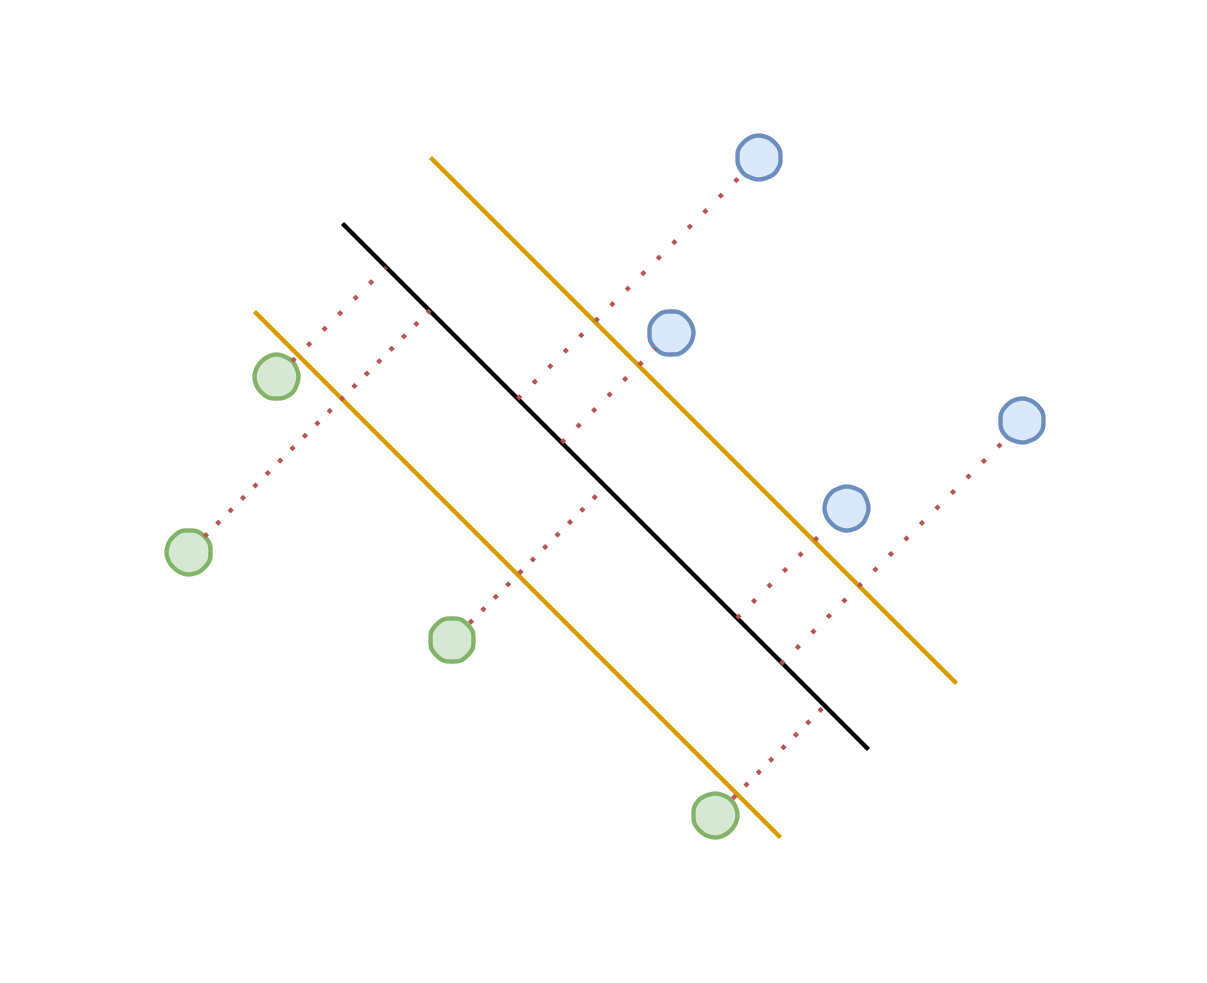
\includegraphics[width=1\textwidth]{Figures/SVM_idea.drawio.png}
    \caption*{Source: Author}
    \label{fig:svm}
\end{figure}


The idea is to find the hyperplane that maximizes the margin between the two classes.
This implies that the hyperplane actually depends only on the support vectors which are the points
closest to the hyperplane. This can be relatively easily reformulated
into a regression problem by using the same idea but instead of classifying the points
we are predicting the distance from the hyperplane. This is called the support vector regression.
Note that the example in Figure \ref{fig:svm} represents a problem that is linearly separable
which is often not the case in practice and there are two remedies how to fix that.
The first one is the usage of the kernel trick which is a way to transform the data into a higher dimensional space
where the data is linearly separable. The second one is to use the \ac{SVM} with a soft margin which is
what most of the \ac{SVM} implementations do. That allows us to set a hyperparameter that allows
some points to be missclasified and acts as a form of regularization where we do not perfectly,
seperate all of the points in the training set. 


The optimization details of the \ac{SVM}s are quite complex and are beyond the scope of this text.
They include the usage of the Lagrange multipliers and the dual optimization problem. The description
of the kernel trick is not included as we opted for the linear kernel in our experiments.
We thus refer the readers to some traditional \ac{ML} textbooks such as \citep{bishop2006pattern}.
The \ac{SVM}s represent a middle ground between the traditional \ac{LR} model and the deep learning models.


\section{\acl{LSTM} \acl{RNN}s}

\acl{RNN}s could be regarded as the state of the art in time series forecasting.
Their architecture allows them to process long sequential data
of theoretically arbitrary length. They can capture the temporal dependencies
in the data and learn sequential patterns. However, the traditional \ac{RNN}s
suffer from the vanishing gradient problem which makes them unable to learn 
long term dependencies. This problem arises
due to the fact that the neurons in \ac{RNN}s are connected to themselves
which makes them multiply the same weight matrix multiple
times which can lead to the fact that the gradient becomes extremely small if the 
weights are small. This is the reason why the \ac{LSTM} cell was
introduced by Hochreiter and Schmidhuber in 1997 \citep{Hochreiter1997}.
The idea is to make the errors constant through time by introducing few improvements
to the original \ac{RNN} cell.

\begin{figure}[!h]
    \centering
    \caption{\acl{RNN} Architecture unwinded in time 
    is feeding outputs back into itself.}
    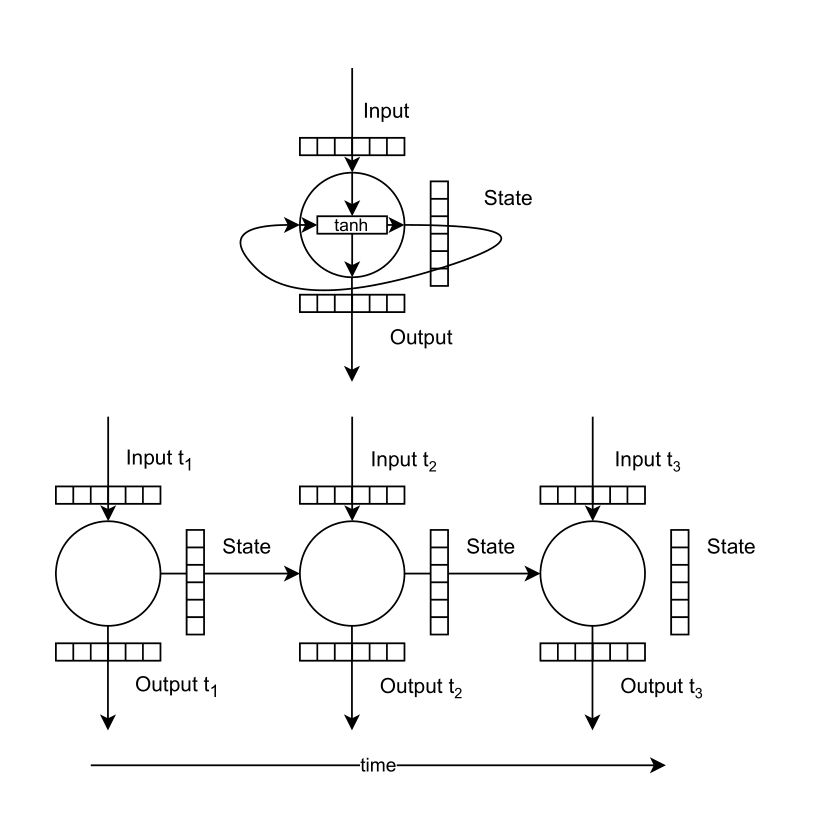
\includegraphics[width=1\textwidth]{Figures/RNN.drawio.png}
    \caption*{Source: Author}
    \label{fig:rnn_architecture}
\end{figure}

The name \acl{RNN} comes from the fact that the cell is able
to feed backward into iself its internal state. Conceptually, this is a kind
of memory or an internal representation of the data. Output in the next
time step is the combination of the current input and the internal state
of the cell usually weighted using the tanh activation function. 
It is a common practice to represent \ac{RNN}s as a chain of cells 
unwined in time even though it is actually a single cell that is fed back into itself.
It is possible to combine multiple such layers of these cells to create
a deep \ac{RNN} which is able to capture more complex patterns in the data.



Despite the promising idea of \ac{RNN}s, they suffer from many training problems.
Multiple remedies have been proposed to fix these problems such as the \ac{LSTM} cell
or the gated recurrent unit cell which are giving the model the ability to learn
long term dependencies.

Since the introduction of the \ac{LSTM} cell, many improvements have been made to the original
architecture we will describe the improved architecture from \citep{Gers2000} which
adds the forget gate to the original architecture. 

\newpage
\begin{figure}[!h]
    \centering
    \caption{\ac{LSTM} cell enables 
    consistent long term memory and stabilizes the training process.}
    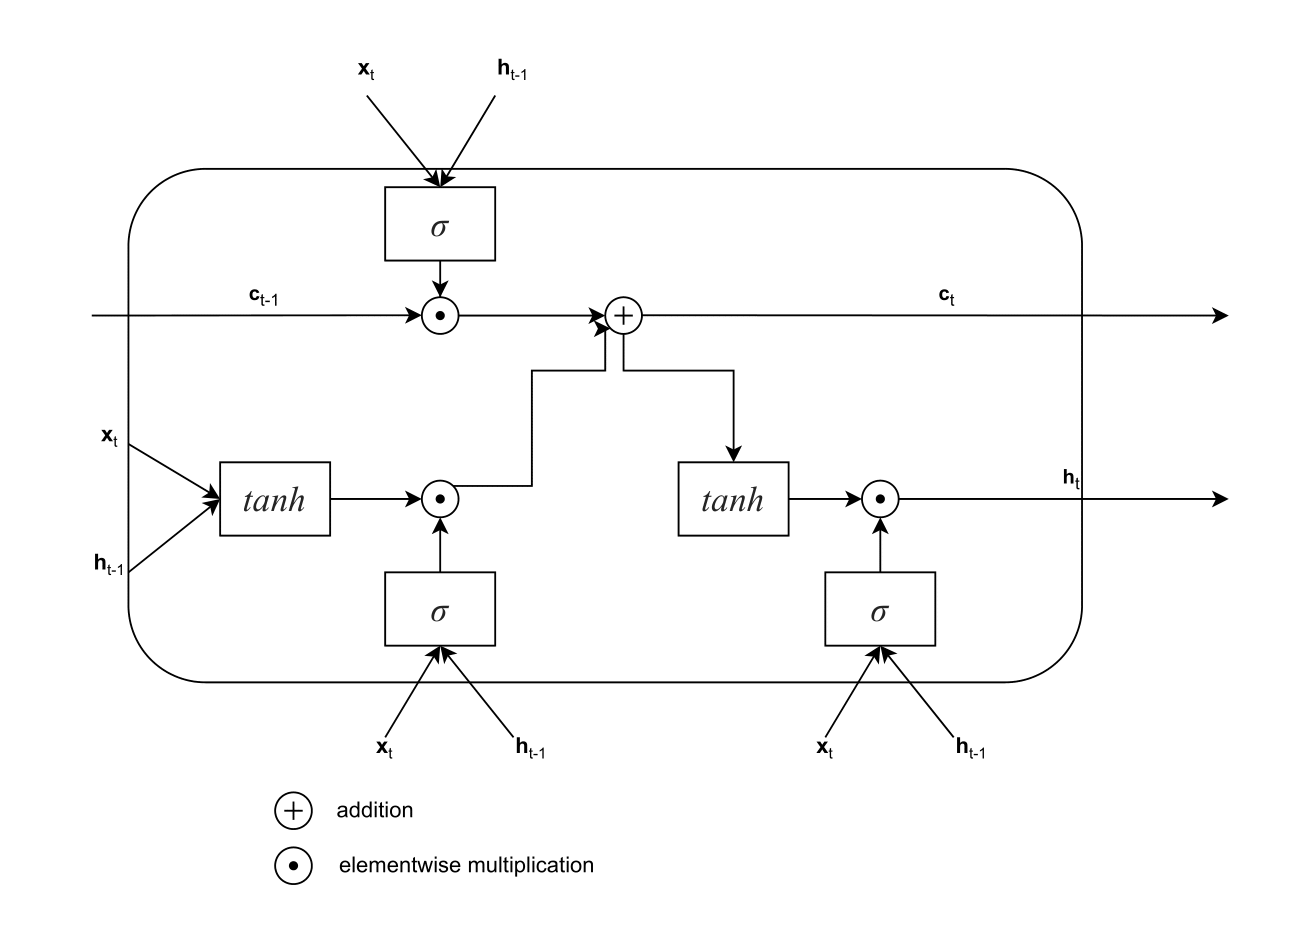
\includegraphics[width=1\textwidth]{Figures/LSTM.drawio.png}
    \caption*{Source: Author}
    \label{fig:lstm_cell}
\end{figure}


\afterpage{
\begin{equation}
    i_t = \sigma \left( \mathbf{W}^i x_t + \mathbf{V}^i h_{t-1} + \mathbf{b}^i \right)
\end{equation}

\begin{equation}
    f_t = \sigma \left( \mathbf{W}^f x_t + \mathbf{V}^f h_{t-1} + \mathbf{b}^f \right)
\end{equation}

\begin{equation}
    o_t = \sigma \left( \mathbf{W}^o x_t + \mathbf{V}^o h_{t-1} + \mathbf{b}^o \right)
\end{equation}

\begin{equation}
    c_t = f_t \odot c_{t-1} + i_t \odot \tanh \left( \mathbf{W}^y x_t + \mathbf{V}^y h_{t-1} + \mathbf{b}^y \right)
\end{equation}

\begin{equation}
    h_t = o_t \odot \tanh(c_t)
\end{equation}
}

The \ac{LSTM} cell consists of three gates: the input gate, the forget gate, and the output gate.
The input gate decides which input information is useful for the cell state. 
The forget gate decides which information to forget from the long term memory.
And finally the output gate decides which information should be passed to the next state.
The exact formulas are given in equations 4.4-4.8 where $\mathbf{W}, \mathbf{V}$ 
represent respective weights of the layers and $\mathbf{b}$ is the bias term. 
We can see that this architecture allows the cell to represent long term
memory as the vector $\textbf{c}$ and short term memory
as the vector $\textbf{h}$ as normal \ac{RNN}s do. 







\section{\acl{PCA}}

\ac{PCA} is a widely used dimensionality reduction technique that is able
to reduce number of dimensions for the purpouses of visualization, noise reduction, and
reduction of the curse of dimensionality. The curse of 
dimensionality refers to the observation that with increasing number of 
dimensions the volume of the space increases exponentially and the data points become
extremely sparse leading to enormous distances between training points.
The fact that \ac{PCA} can be used as a noise reduction technique is 
technically a byproduct of the way how this algorithm works. We will start with the
general idea to ilustrate how this concept emerges.


Conceptually, \ac{PCA} can be thought of in two ways: maximum variance formulation
and minimum reconstruction error formulation. We will follow with the maximum variance formulation.
The idea is to find the hyperplane that maximizes the variance of the data projected onto it.
Refer to Figure \ref{fig:pca} for the illustration of the concept. We can see
that the first principal component is the line that maximizes the variance of the projection
of the data onto it. The second principal component captures
less variance and is orthogonal to the first principal component. \ac{PCA} can
generally create as many principal components as there are dimensions in the data.
This means that for \textit{n} dimensions we can create \textit{n} principal components which
are orthogonal to each other and are odered by the amount of variance they capture. 
Finally we can reduce the number of dimensions by projecting the data onto the first \textit{k} principal components
where \textit{k} is the number of dimensions we want to keep or the desired variance 
we want to preserve.

\begin{figure}[!h]
    \centering
    \caption{\ac{PCA} projection where the red line
    is representing the variance maximizing hyperplane. All of the 
    principal components are orthogonal to each other.}
    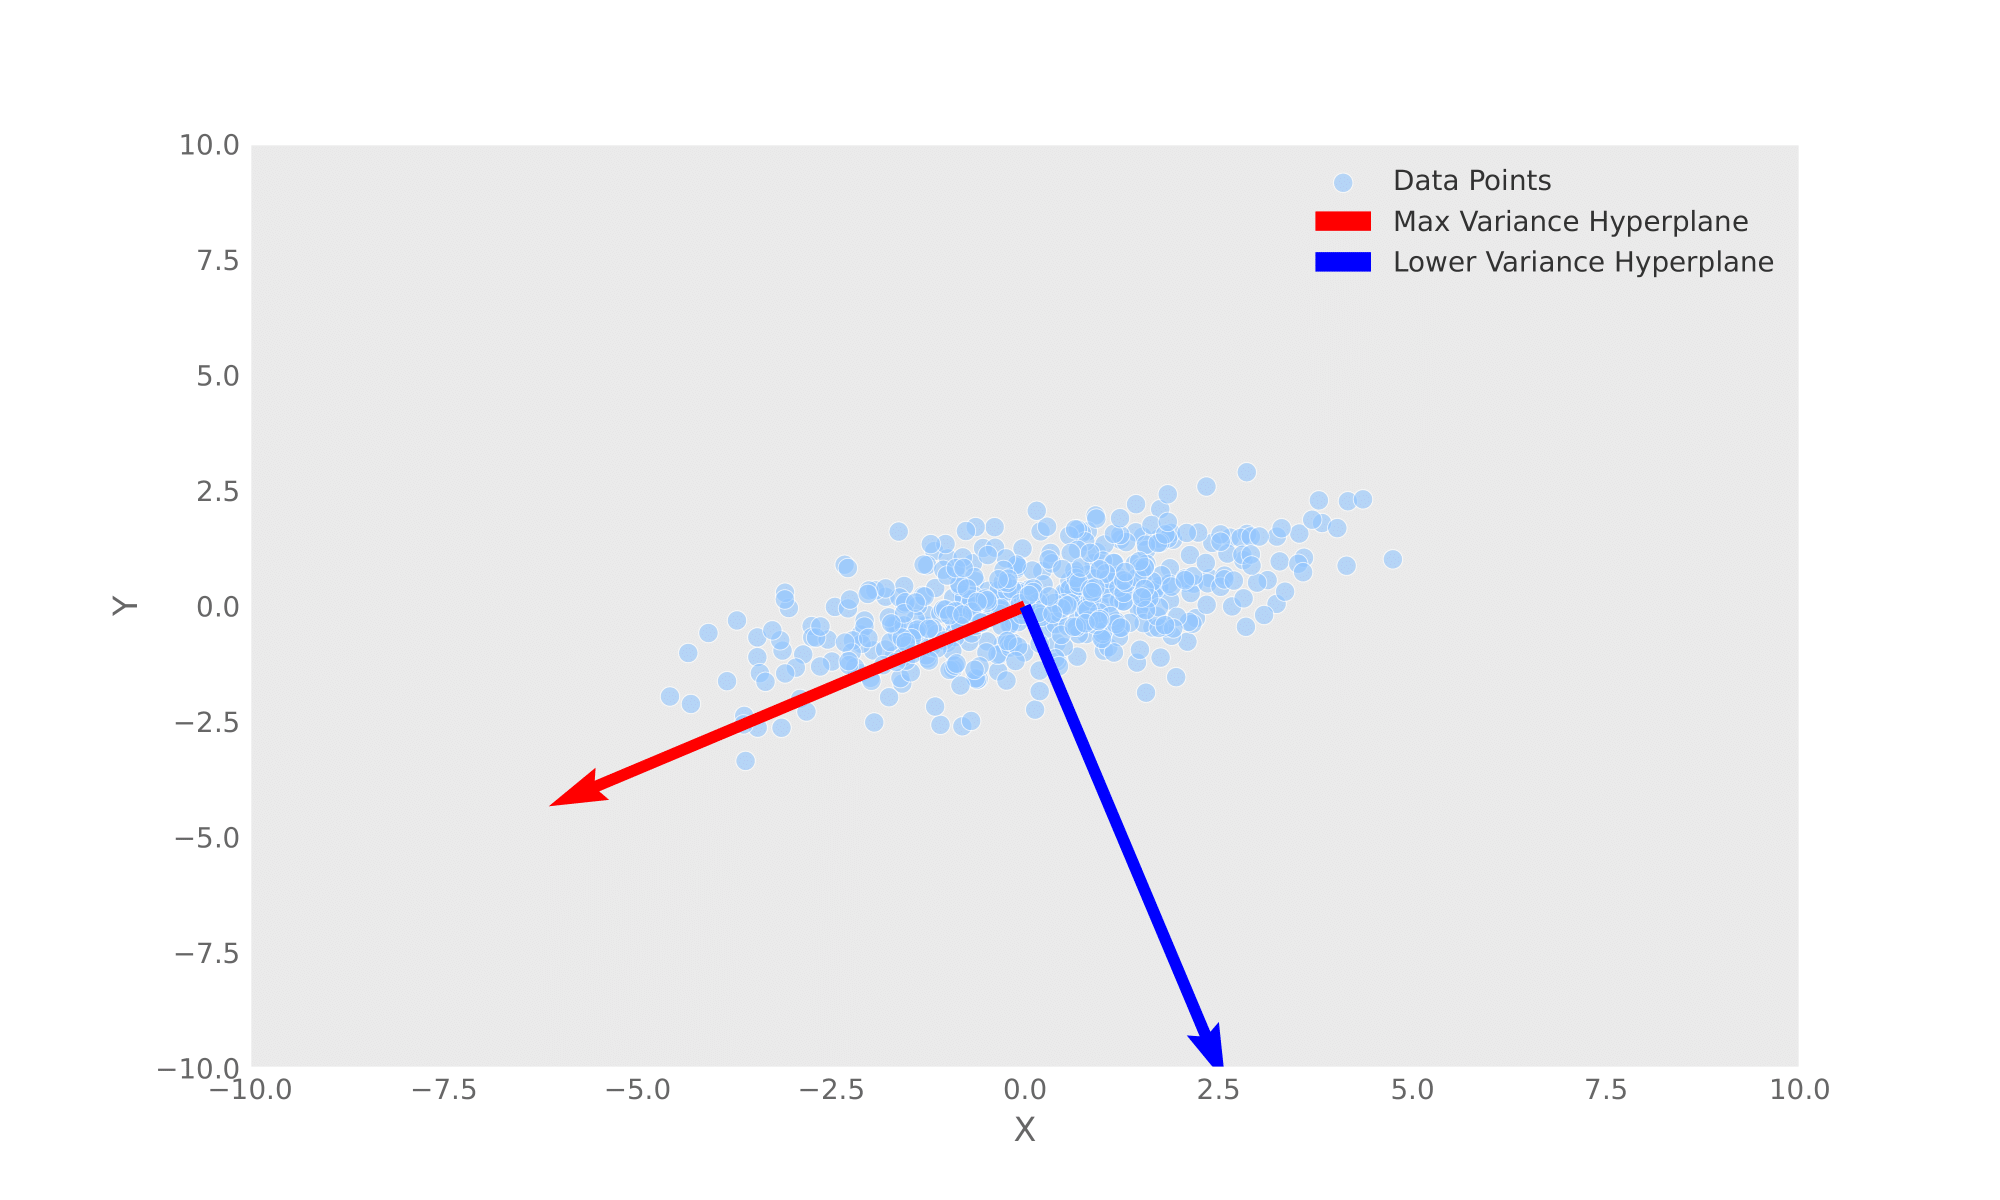
\includegraphics[width=1\textwidth]{Figures/pca_plot.png}
    \caption*{Source: Author}
    \label{fig:pca}
\end{figure}

This is where the idea that \ac{PCA} can be used as a noise reduction technique comes from.
As this algorithm keeps only data which captures most of the variance
and theoretically should drop information that is less informative.
It is interesting to note that as the principal components are orthogonal to each other 
they are also uncorrleated which is a useful property for many \ac{ML} algorithms. 
We acknowledge that \ac{PCA} is not in itself a noise reduction technique
but it is a rather elegant and simple way that sometimes reduces noise in the data.
The implementation details of \ac{PCA} are beyond the scope of this text but we refer the readers
to the original paper \citep{Pearson1901}.




\section{Stationarity in Time-Series}

We would like to explicitly adress the concept of stationarity as there 
seems to be a lot of confusion around the topic especially because the boundary between 
traditional econometric models and machine learning models is not always clear.

Stationarity is a crucial concept in time-series analysis. Despite the fact, that there exist
many tests and rigid definitions for it, it is often reduced to the 
concept of constant mean and variance or generally to the fact that the parameters
of the distribution do not change in time. Without this property the errors
of the model become function of time which is not desirable for proper inference.

Econometrics usually prefers stationary data for aforementioned reasons because it 
is cruicial for inference and interpretation of the results. That is 
why econometricians like to model returns instead of prices, as returns
should generally be stationary. Imporantly, there is always the possibility
to transform the predictions back to the original prices by adding the forecasted
returns to the last observed price and potentially reversing some normalization steps.

This is different for \ac{ML} as the focus is on prediction and the models are fundamentally 
different. As the models are trained using gradient descent and not using the
analytical solutions, the stationarity is not as crucial. Clearly, 
the models will perform better on stationary data because it requiers much 
less capacity for the model as some of the information removed by differencing.
However, models with enough capacity can easily learn non-stationary data and
capture information about trends, seasonalities, and other patterns. 
Thus we decided to test our models on both prices directly and on returns where
the results are much less dependent on changes in the distribution of the data.

\section{Proposed Forecasting Framework}

We propose a forecasting framework which is designed to compare the performance between using \ac{PCA} as a 
dimensionality reduction technique and using the raw data. 
The framework is shown in Figure \ref{fig:forecasting_framework}.
The preprocessing layer is responsible for cleaning the data, filling in missing values and tranforming 
the problem to supervised learning as described 
in \ref{chap:three}. Following stage is responsible for reducing the number of features. 
The first \ac{PCA} step transforms the data onto \textit{n} principal components and the filtering step
chooses the most important features such that their cumulative variance adds up to 95\%, 98\% or 99\%.
As decreasing the dimensionality would completely change the desired
complexity of the algorithms and the differences might be attributed only to the change 
of dimensionality we upsample the data back to the original dimensionality using 
the inverse transformation of the \ac{PCA} algorithm.

Following is the \ac{LSTM} reshaping layer that is responsible for transforming the data into a 3D tensor for 
the \ac{LSTM} \ac{RNN} as described 
in \ref{chap:three}. The most crucial layer is the forecasting layer that essentially consists of 3 parts.
Firstly, it normalizes the variables using robust scaler to ensure that the input features come from 
the same value range. Secondly, it uses grid search to search for the best
hyperparameters for the model. 
Lastly, it trains the model and evaluates the performance using the best found model. This is the reason
why we abstract the metrics layer seperately to make it apparent that the metrics are calculated
on the best model found by the grid search. The metrics layer is also the layer where
we can statistically compare the significance of the difference between the models.
It is important to note that this framework is executed across all specified forecasting models, 
cryptocurrencies of interest, and forecasting horizons as we expect the effects
to be quite different for different models and forecasting horizons. 


As we have already noted the fact that that the target price is clearly non-stationary,
has important implication for the choice of splitting strategy for the grid search 
hyperparameter optimization. 
There are two main strategies for splitting the data into training and testing sets.
The first one is traditional train, development, and test split where the model is trained on the training set,
hyperparameters are optimized on the development set, and the model is evaluated on the test set.
This approach is generally sufficient when the dataset is large enough and we believe
that the distributions of the three datasets are similar. 
A more robust approach is to use grid search with cross-validation. 
This approach makes sure that we have not overfitted the model to the development set.
Firstly, we split the data into training and testing set. And then 
we iteratively split the training set into training and validation set. 
Train the model on the training part of the train set and evaluate on the validation set.
Finally we average over the results across all validation sets and take the best hyperparameters
from the provided grid. This approach avoids overfitting and is typically
used when we have enough compute to train the models. 


Note that the goal of grid search is to create a robust representation of a 
reasonable test set distribution as it samples randomly the points into the training and validation set.
This approach works if the data is stationary and the distribution of the data does not change drastically in time.
But time series rarely have this property and cryptocurrencies suffer especially profound changes in the distribution
as they have grown in popularity. The difference between the training and test set
is extreme but that is something that we can do very little about as we want the test set
to be as close to the future as possible. 


Additionally, there is an extremely
common mistake that researchers make when they use grid search for time series data.
This problem is called data leakage and it occurs when future distribution of the data
is used to optimize the hyperparameters. As \ac{ML} models typically 
require data to be scaled and normalized, the parameters for the normalization 
need to be learned only on the historical data not on the future data otherwise the 
results will be biased and suggest higher quality of the model than it actually is.
Theoretically, this could be relaxed on the training set as the normalization
might be fitted on the whole training set but it is crucial that the test set distribution
is never leaked to the fitting procedure. However, we believe that
the correct methodology is to use a rolling window approach for the grid search
where the normalization parameters are fitted on the training part of the train set
correctly distributed in time.
This is why we use time series split for the grid search without randomly shuffling the data.
This approach splits the training set into \textit{k} folds and iteratively
trains the model on \textit{k-1} folds and evaluates on the \textit{k-th} fold.
This approach has the advantage that the model is actually trained with
different sized training sets which is useful for generalization properties
but has the disadvantage that the difficulty of the splits is extremely volatile.
This is definitely a limitation as the performances between splits
can vary significantly and averaging over the results might be prone to noise.
However, we believe that this is the methodologically correct approach.
\begin{figure}[!h]
    \centering
    \caption{Time Series Split with \textit{k=2} incrementally
    increases the training set size and leads to different cross 
    validation training split sizes.} 
    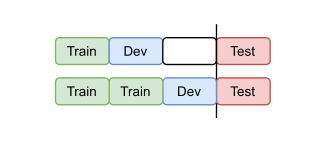
\includegraphics[width=1\textwidth]{Figures/time_series_split.drawio.png}
    \caption*{Source: Author}
    \label{fig:ts_split}
\end{figure}
We opted to use only two splits as the the data size
is relatively small and the results were extremely noisy when using
more splits.


\begin{figure}[!h]
    \centering
    \caption{Proposed Forecasting Framework conists of 
    four independent sequential layers.}
    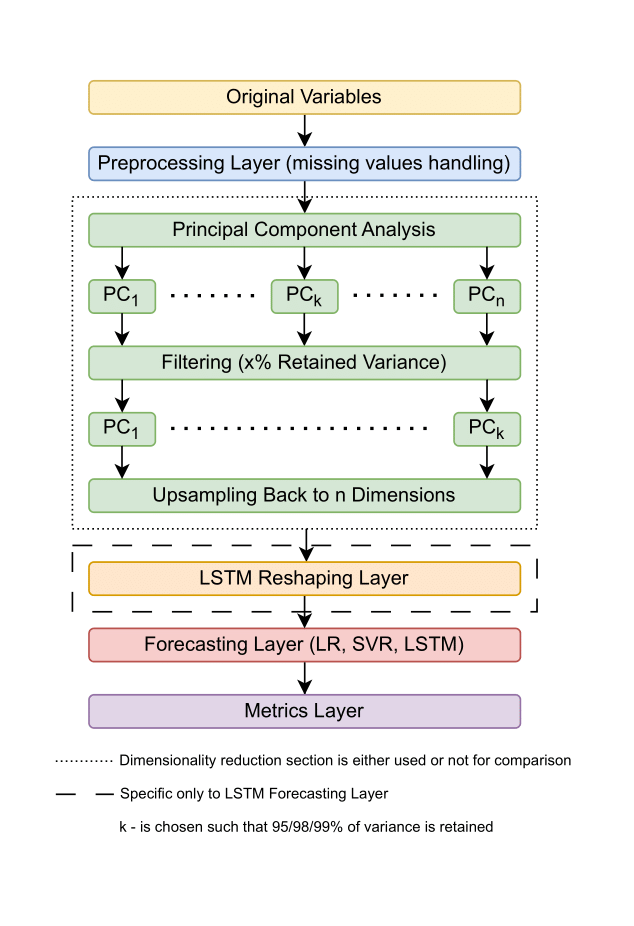
\includegraphics[width=1\textwidth]{Figures/Forecasting_framework.drawio.png}
    \caption*{Source: Author}
    \label{fig:forecasting_framework}
\end{figure}